
%%%%%%%%%%%%%%%%%%%%%%% file typeinst.tex %%%%%%%%%%%%%%%%%%%%%%%%%
%
% This is the LaTeX source for the instructions to authors using
% the LaTeX document class 'llncs.cls' for contributions to
% the Lecture Notes in Computer Sciences series.
% http://www.springer.com/lncs       Springer Heidelberg 2006/05/04
%
% It may be used as a template for your own input - copy it
% to a new file with a new name and use it as the basis
% for your article.
%
% NB: the document class 'llncs' has its own and detailed documentation, see
% ftp://ftp.springer.de/data/pubftp/pub/tex/latex/llncs/latex2e/llncsdoc.pdf
%
%%%%%%%%%%%%%%%%%%%%%%%%%%%%%%%%%%%%%%%%%%%%%%%%%%%%%%%%%%%%%%%%%%%


\documentclass[runningheads,a4paper]{llncs}

\usepackage{amssymb,amsmath}
\setcounter{tocdepth}{3}
\usepackage{graphicx}
\usepackage{enumitem}
\usepackage{url}

\begin{document}

\mainmatter  % start of an individual contribution

% first the title is needed
\title{Parallel Multipoint Approximation Method for Large Scale Optimization Problems 
\thanks{This study was supported by the Russian Science Foundation, project No. 16-11-10150.}}

% a short form should be given in case it is too long for the running head
\titlerunning{Parallel Multipoint Approximation Method}

\author{ Victor P. Gergel%(ORCID 0000-0002-4013-2329)
$^1$ \and
Konstantin A. Barkalov%(ORCID 0000-0001-5273-2471)
$^1$ \and
Evgeny A. Kozinov%(ORCID )
$^1$ \and
Vassili V. Toropov%(ORCID 0000-0002-7017-5055)
$^{1,2}$
}
%
\authorrunning{V.P. Gergel \and K.A. Barkalov \and E.A.Kozinov \and V.V. Toropov}
% (feature abused for this document to repeat the title also on left hand pages)

% the affiliations are given next; don't give your e-mail address
% unless you accept that it will be published
\institute{$^1$Lobachevsky State University of Nizhny Novgorod, Nizhny Novgorod, Russia\\
\email{\{victor.gergel, konstantin.barkalov, evgeny.kozinov\}@itmm.unn.ru}\\
$^2$Queen Mary University of London, London, UK\\
\email{v.v.toropov@qmul.ac.uk}\\
}

%
% NB: a more complex sample for affiliations and the mapping to the
% corresponding authors can be found in the file "llncs.dem''
% (search for the string "\mainmatter" where a contribution starts).
% "llncs.dem" accompanies the document class "llncs.cls".
%

%\toctitle{Lecture Notes in Computer Science}
%\tocauthor{Authors' Instructions}
\maketitle

\begin{abstract}
TBD

\keywords{design optimization, multidisciplinary optimization, multipoint approximation method, parallel computing.}
\end{abstract}

\section{Introduction}
TBD

In problems with a large (in the order of hundreds) number of design variables, the multipoint approximation method (MAM \cite{Toropov1989,Toropov1992,ToropovFilatov1993}) proved to be efficient, e.g. in turbomachinery applications \cite{ShahparPolynkinToropov2008,PolynkinToropovShahpar2008,PolynkinToropovShahpar2010} . This method is an iterative optimization technique based on mid-range approximations built in trust regions. A trust region is a sub-domain of the design space in which a set of design points, produced according to a small-scale design of experiments (DoE), are evaluated. These and a subset of previously evaluated design points are used to build metamodels of the objective and constraint functions that are considered to be valid within a current trust region. The trust region will then translate and change size as optimization progresses. The trust region strategy has gone through several stages of development to account for the presence of numerical noise in the response function values \cite{KeulenToropovMarkine1996,ToropovKeulenMarkine1996} and occasional simulation failures \cite{ToropovMarkineHolden1999}. The mid-range approximations used in the trust regions, as originally suggested in \cite{Toropov1989} for structural optimization problems, are intrinsically linear functions (i.e. nonlinear functions that can be led to a linear form by a simple transformation) for individual sub-structures, and assembly of them for the whole structure. This was enhanced by the use of gradient-assisted metamodels \cite{ToropovFilatov1993}, use of simplified numerical models that is also termed a multi-fidelity approach,\cite{ToropovMarkine1996} and the use of analytical models derived by Genetic Programming \cite{ToropovAlvarez1998}. One of the recent developments \cite{PolynkinToropov2012} involved the use of approximation assemblies, i.e. a two stage approximation building process that is conceptually similar to the original one used in \cite{Toropov1989} but is free from the limitation that lower level approximations are linked to individual substructures.

The Moving Least Squares Method (MLSM) was proposed in \cite{LancasterSalkauskas1981} for smoothing and interpolation of scattered data and later used in the mesh-free form of the FEM \cite{Liszka1984}. As suggested in \cite{ChoiYounYang2001}, it can be used as a technique for metamodelling and used in MDO frameworks. The MLSM is a weighted least squares method where the weights depend on the Euclidean distance from a sample point to where the surrogate model is to be evaluated. The weight value for a certain sample point decays as the distance increases. Describing the weight decay with a Gaussian function tends to be the most useful option even though many others have been evaluated in \cite{ToropovSchrammSahaiJones2005}. As demonstrated in \cite{PolynkinToropov2010}, the cross-validated MLSM can be used both for design variable screening and for surrogate modelling. In order to create an efficient MDO framework for problems with disparate discipline attributes \cite{OllarToropovJones2014} extended the optimization approach of MAM to the use of local DOEs and MLS approximations built in different subspaces of the total design variable space corresponding to the individual disciplines. The subspaces are finally combined into the total design variable space in which the resulting MDO problem is solved.

TBD

\section{The Multipoint Approximation Method}
\label{sec:MAM}

It is useful to start with a brief description of MAM. A typical formulation of a constrained optimization problem that MAM works with is as follows:
\begin{equation}
  \label{eq:problem}
  \begin{array}{c}
  \min\limits_{a_i \le x_i \le b_i}F_0(x) \\
  s.t.\; F_j(x) \le 1,\; j=1,\dots ,M,
  \end{array}
\end{equation}
where $x$ is the vector of design variables, $a$ and $b$ are the lower and upper bounds for the design variables, respectively, $F_0(x)$ is the objective function, and $F_j(x)$ are the constraints. The numbers of design variables and constraints are $n$ and $M$, respectively. MAM attempts to solve this problem by using approximations of the objective function and constraints in a series of trust regions. The trust region strategy seeks to zoom in on the region where the constrained minimum is achieved. It aims at finding a trust region that is sufficiently small for the approximations to be of sufficiently good quality to improve the design, and that contains the point of the constrained minimum as its interior point. The main loop of the MAM is organized as follows.

Algorithm (MAM).
\begin{enumerate}
\item Initialization: choose a starting point $ x^0$ and initial trust region $[ a^0,  b^0]$ such that $ x^0 \in [ a^0,  b^0]$.
\item At the $k$-th iteration the current approximation to the constrained minimum is $ x^k$, the current trust region is $[ a^k,  b^k] \subset [ a^0,  b^0]$.
  \begin{enumerate}[label=(\alph*)]
    \item Design of Experiments (DoE): a set of points $ x_k^i \in [ a^k,  b^k]$ is chosen to be used for approximation building. Responses are evaluated at the DoE points and approximations are built using the obtained values. Currently, the pool of approximation methods available in MAM consists of a metamodel assemblies \cite{PolynkinToropov2012} and the moving least-squares metamodels \cite{LancasterSalkauskas1981,Liszka1984,ChoiYounYang2001,ToropovSchrammSahaiJones2005}. Other metamodel types could be used as well.

    Denote the approximate objective function and constraints by $\widetilde{F}^k_0(x)$ and $\widetilde{F}^k_j(x)$, respectively.
    \item The original optimization problem (\ref{eq:problem}) is replaced by the following problem:
    \begin{equation}
      \label{eq:problem_approx}
      \begin{array}{c}
      \min\limits_{a_i^k \le x_i ^k\le b_i}\widetilde{F}^k_0(x) \\
      s.t.\; \widetilde{F}^k_j( x) \le 1,\; j=1,\dots ,M,
      \end{array}
    \end{equation}
    The approximate problem (\ref{eq:problem_approx}) is solved using Sequential Quadratic Programming (SQP) and the solution of this problem determines the center of the next trust region.
    \item The size of the next trust region is determined depending on the quality of approximations at the previous iteration, on the history of the points $ x^k$, and on the size of the current trust region \cite{KeulenToropovMarkine1996}.
    \item The termination criterion is checked (it is a part of the trust region strategy and depends on the position of the point $ x^{k+1}$ in the current trust region, the size of the current trust region and the quality of approximations). If the termination criterion is satisfied, the algorithm proceeds to step 3. Otherwise, it returns to step 2.
  \end{enumerate}
  \item Optimization terminates. The obtained approximation to the solution of the problem (\ref{eq:problem}) is $ x^{k+1}$.
\end{enumerate}

The selection of the approximations $\widetilde{F}^k_j(x),\; j=0, \dots ,M,$ is such that their evaluation is inexpensive as compared to the evaluation of the original response functions $F_j(x)$. For example, intrinsically linear functions were successfully used for a variety of design optimization problems in the works \cite{ToropovFilatov1993,KeulenToropov1997}. The approximations are determined by means of the weighted least squares:
\begin{equation}\label{eq:least_sq}
\min \sum_{p=1}^P{w_{pj}\left[ F_j(x_p)- \widetilde{F}^k_j(x_p,a_j) \right]^2}.
\end{equation}
In (\ref{eq:least_sq}) minimization is carried out with respect to the tuning parameters $a_j$; $w_{pj}$ are the weight coefficients, and $P$ is the number of sampling points in Design of Experiments (DoE) which must not be less than the number of parameters in the vector $a_j$.

The weight coefficients $w_{pj}$ strongly influence the difference in the quality of the approximations in different regions of the design variable space. Since in realistic constrained optimization problems the optimum point usually belongs to the boundary of the feasible region, the approximation functions should be more accurate in such domain. Thus, the information at the points located near the boundary of the feasible region is to be treated with greater weights. In a similar manner a larger weight can be allocated to a design with a better objective function, see \cite{ToropovFilatov1993,KeulenToropov1997}.

As optimization steps are carried out, a database with response function values becomes available. In order to achieve good quality approximations in the current trust region, an appropriate selection of DoE points must be made. In this work, DoE points in each trust region is generated randomly. Generally, points located far from the current trust region would not contribute to the improvement of the quality of the resulting approximations in the trust region. For this reason only points located in the neighborhood of the current trust region are taken into account.%, as depicted in Fig. 1.
A box in the space of design variables, which is approximately 1.5 to 1.8 times larger than the box representing the current trust region, was found by numerical experimentation to be a reasonable choice for the size of the neighborhood.

In this work an approach is used that is based on the assembly of different approximate models $\{\varphi_l\}$ into one metamodel using the following form (note that the indices $j$ and $k$ are suppressed to simplify notation):
\begin{equation}\label{eq:assembly}
\widetilde{F}(x) = \sum_{l=1}^{NF}{b_l\varphi_l(x)},
\end{equation}
where $NF$ is the number of regressors in the model pool $\{\varphi_l\}$ and $b_l$ are corresponding regression coefficients.
The used procedure consists of two subsequent steps. In the first step, the parameters $a_l$ of individual functions (regressors) $\varphi_l$ in (\ref{eq:assembly}) are determined by solving a weighted least squares problem using a specified a DoE of $P$ points:
%\begin{equation}\label{eq:least_sq}
\[
\min \sum_{p=1}^P{w_{p}\left[ F(x_p)- \varphi_l(x_p,a_l) \right]^2},
\]
%\end{equation}
where minimization is carried out with respect to the tuning parameters $a_l$.

In the second step, based on the same DoE and keeping the obtained parameters $a_l$ fixed, a vector $b$ in (\ref{eq:assembly}) is estimated using the following formulation
\[
\min \sum_{p=1}^P{w_{p}\left[ F(x_p)- \widetilde{F}(x_p,b) \right]^2},
\]
that leads to solving a linear system of $NF$ equations with $NF$ unknowns $b_l$, where $NF$ is the number of regressors in the model pool $\{\varphi_l\}$.


\section{Parallel Algorithm}
\label{sec:par_alg}

\section{Numerical Example}
\label{sec:num_example}

The example considered in this study is a classical engineering optimization problem known as the scalable cantilevered beam \cite{Vanderpllaats2001}. The engineering object to be optimized is shown in Fig. \ref{fig:beam} taken from \cite{Vanderpllaats2001}.

\begin{figure}[ht]
    \centering
    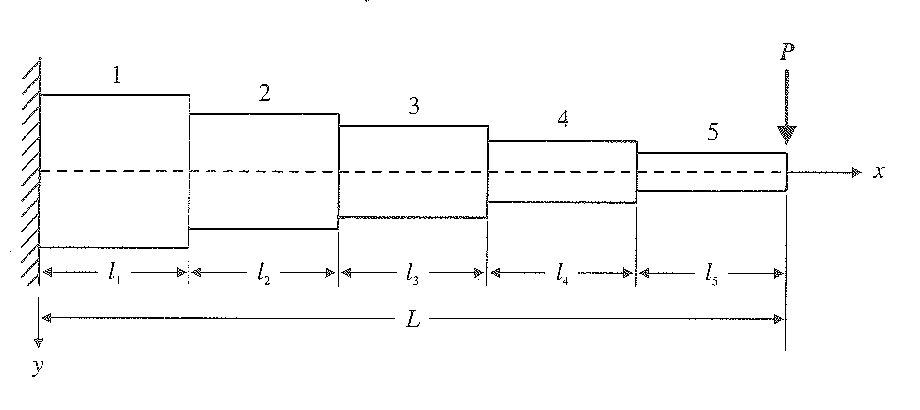
\includegraphics[width=1.0\textwidth]{beam.png}
    \caption{The cantilevered beam}
    \label{fig:beam}
\end{figure}

The design variables are the widths $b_i$ and heights $h_i$ of the segments. The number of segments $N$ can be chosen arbitrary. The total length of the beam is 500 cm, the lengths of the segments are $l_i=500/N$  cm. There are $N$ geometric constraints (the aspect ratios of each block (i.e. heights divided by widths) should not exceed 20) and $N$ constraints on the stress, calculated at the left end of each segment (stresses should not exceed  $\bar{\sigma}=14000\; N/cm^2$). There is also also a constraint on the displacement at the tip, which should not exceed 2.5 cm. The load is $P = 50 000\; N$, the Young's modulus is $E=2\cdot 10^7  N/cm^2$.

The deflection $y_i$ at the right hand of the $i$-th segment is given by the following recursive formulas:
\begin{displaymath}
  \begin{array}{c}
    y_0=y_0'=0, \\
    y_i'=\frac{P\cdot l_i}{E\cdot I_i}\Big[ L+\frac{l_i}{2}-\sum\limits_{j=1}^i l_j\Big]+y_{i-1}', \\
    y_i=\frac{P\cdot l_i^2}{2E\cdot I_i}\Big[L-\sum\limits_{j=1}^i l_j + \frac{2l_i}{3}\Big]+y_{i-1}'l_i+y_{i-1}.
  \end{array}
\end{displaymath}
The moment of inertia of a segment is $I_i=\frac{b_i h_i^3}{12}$ and the bending moment at the left end is $M_i=P[L+l_i- \sum_{j=1}^{i}  l_j ]$. The maximum bending stress in the segment $i$ is then given by the following formula:
\begin{displaymath}
  \sigma_i=\frac{M_i h_i}{2I_i}
\end{displaymath}

We are looking for a design with smallest volume $V = \sum_{i=1}^N b_i h_i l_i$. The widths $b_i$ vary from 1.0 to 10.0 cm and the heights $h_i$ from 5.0 to 100.0 cm. The optimization problem is formulated as follows:
\begin{displaymath}
  \begin{array}{c}
    \min\limits_{ b,  h}V( b,  h) \\
    s.t.\;1.0\le b_i \le 10.0, \\
    5.0 \le h_i \le 100.0, \\
    y_N\le 2/5, \\
    \sigma_i \le \bar{\sigma}=14000, \\
    \frac{h_i}{b_i}\le 20.
  \end{array}
\end{displaymath}

With $N=50$ segments (corresponding to 100 design variables) the SQP solution of this problem is $V = 63704.598\; cm^3$. MAM obtained the solution $V = 63935.360\; cm^3$, using 1500 function evaluations (as compared to almost 8000 evaluations used by SQP). The number of points in a trust region used to build approximations was 150. The solution obtained by MAM is very close to the reference solution obtained by SQP, except for the last design variable (the height of the last segment), which indicates that the problem is insensitive to this variable near the optimum, making it hard for the metamodels to capture this dependence. Both SQP and MAM solutions are, however, feasible and differ only slightly in the value of the objective function.


\section{Conclusions}


\bibliography{bibliography}{}
\bibliographystyle{nature}



%\bibitem{Strongin2000}
%Strongin, R.G., Sergeyev, Y.D.: Global Optimization with Non-Convex Constraints. Sequential and Parallel Algorithms. Kluwer Academic Publishers, Dordrecht (2000); DOI: 10.1007/978-1-4615-4677-1
%
%\bibitem{Barkalov2002}
%Barkalov, K.A., Strongin, R.G.: A global optimization technique with an adaptive order of checking for constraints. Comput. Math. Math. Phys. 42(9), 1289--1300 (2002)
%
%\bibitem{Gergel2005}
%Gergel, V.P., Strongin, R.G.: Parallel computing for globally optimal decision making on cluster systems. Future Gener. Comput. Syst. 21(5), 673--678 (2005); DOI: 10.1016/j.future.2004.05.007
%
%\bibitem{Strongin2013}
%Sergeyev, Ya.D., Strongin, R.G., Lera, D.: Introduction to global optimization exploiting space-filling curves. Springer (2013);  DOI: 10.1007/978-1-4614-8042-6
%
%\bibitem{Barkalov2010}
%Barkalov, K., Ryabov, V., Sidorov, S.: Parallel Scalable Algorithms with Mixed Local-Global Strategy for Global Optimization Problems. In: Hsu, Ch., Malyshkin, V. (Eds.) MTPP 2010, LNCS, vol. 6083, pp. 232--240. Springer, Heidelberg (2010); DOI: 10.1007/978-3-642-14822-4$\_$26
%
%\bibitem{Barkalov2015}
%Barkalov, K., Gergel, V., Lebedev, I.: Use of Xeon Phi Coprocessor for Solving Global Optimization Problems. In: Malyshkin, V. (Ed.) PaCT 2015, LNCS, vol. 9251, pp. 307--318. Springer, Heidelberg (2015); DOI: 10.1007/978-3-319-21909-7$\_$31
%
%\bibitem{Barkalov2016}
%Barkalov, K., Gergel, V.: Parallel Global Optimization on GPU. J. Glob. Optim. 66(1), 3--20 (2016); DOI: 10.1007/s10898-016-0411-y
%
%\bibitem{Gergel2016}
%Barkalov, K., Gergel, V., Lebedev, I.: Solving Global Optimization Problems on GPU Cluster. In: Simos T.E. (Ed.) ICNAAM 2015, AIP Conference Proceedings, vol. 1738, art. no. 400006 (2016); DOI: 10.1063/1.4952194
%
%\bibitem{Gergel2015}
%Gergel, V., Sidorov, S.: A Two-Level Parallel Global Search Algorithm for Solution of Computationally Intensive Multiextremal Optimization Problems. In: Malyshkin, V. (Ed.) PaCT 2015, LNCS, vol. 9251, pp. 505--515. Springer, Heidelberg (2015); DOI: 10.1007/978-3-319-21909-7$\_$49
%

%\end{thebibliography}

\end{document}
